\documentclass{article}
\usepackage[utf8]{inputenc}
\usepackage{amsmath}
\usepackage[a4paper,body={140mm,250mm}]{geometry}

\usepackage{graphicx} 
\usepackage{array} 
\usepackage{newtxtext,newtxmath}
\usepackage[varl]{inconsolata}

\begin{document}
\begin{titlepage}
  \begin{flushleft}\scshape
    Lund University\\
    Automatic Control\\[\smallskipamount]
    FRTN70 Project in Systems, Control and Learning\\
    Spring 2018
  \end{flushleft}
  \vspace*{0pt plus 0.3fill}
  \begin{center}
    \huge \textbf{Ball-Catching Robot}\\[4mm]     
    \large\textbf{Project Plan Group A}\\[5mm]
         Olle Flitig\footnote{\texttt{olle.flitig@student.lu.se}}\quad
         Sara Rask\footnote{\texttt{sara.rask@student.lu.se}}\quad
         Björn Duktig\footnote{\texttt{bjorn.duktig@student.lu.se}}\quad
         Amanda P. Solver\footnote{\texttt{amanda.solver@student.lu.se}}
  \end{center}
\begin{center}
    Project Advisor: Mycke K. Unnig
\end{center}
\vfill
\end{titlepage}        

\section{Project Purpose}
The goal of this project is to make a robot arm that can catch balls based on visual feedback. The work will be based on the PhD-thesis (TFRT-1098) made by Magnus Linderoth.

\section{Equipments and material} \label{sec:equipment}
In this section we propose a list containing the materials needed for the project. We have appended the approximate costs of each item on the list --- based on the research we have been doing online.
\subsection{Robotics}
    \begin{itemize}
        \item Robotic arm metal frame with six degrees of freedom. (approx. 1000 SEK)
        \item MG996R Servo x 4 for movement off the robotic arm. (approx. 80 SEK/each)
        \item MG90S Servo x 2 for movement off the robotic arm. (approx. 80 SEK/each)
        \item Arduino Uno R3 to generate pwm signals to the servos. (approx. 200 SEK)
        \item 5V DC power supply for servos. (approx. 100 SEK)
        \item 12V DC power supply for arduino. (approx. 100 SEK)
    \end{itemize}
\subsection{Ball detection}
    \begin{itemize}
        \item High speed cameras (basler ACA800-200GC) x 2. (approx. 1000 SEK/each)
        \item PoE gigabit switch. (approx. 1000 SEK)
        \item Gigabit ethernet cable x 3. (approx. 100 SEK/each)
    \end{itemize}
%\newpage

\section{Modelling and System Design}
We are proposing the code structure seen in Figure \ref{fig:uml} for our project. Considering a structure using four different packages the project can be split up and developed independently from one another. Furthermore, the packages represent the division of labour proposed in section \ref{sec:division}

\begin{figure}[b] 
	\centering
 	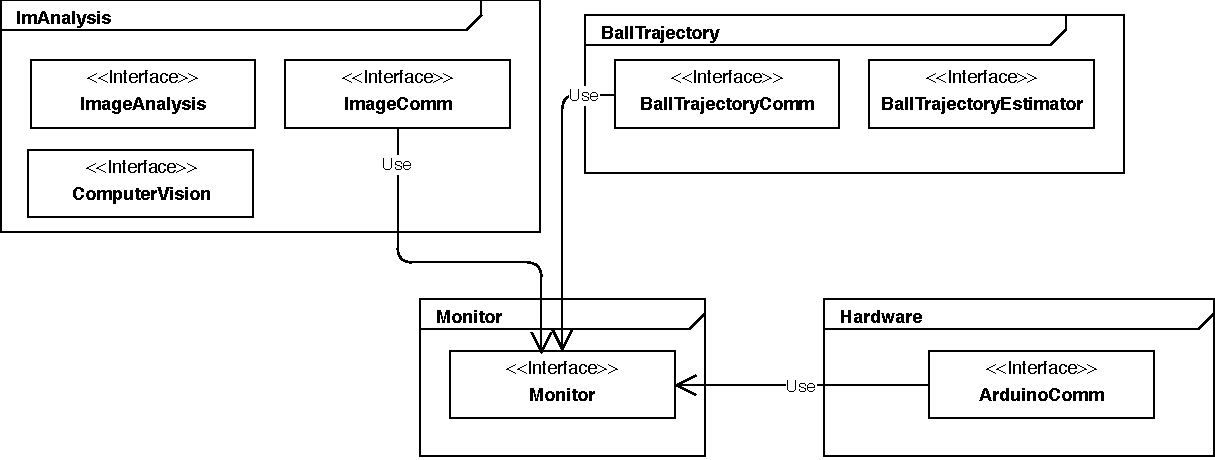
\includegraphics[width=0.85\textwidth]{figures/UML}
    \caption{The structure of the software.}
    \label{fig:uml}
\end{figure}

\noindent
The hardware setup will include:
\begin{itemize}
\item The robot arm.
\item Two cameras mounted behind the robot.
\item An arduino to distribute signals to the servos in the robot arm.
\item A PC to run the software on.
\end{itemize}
The overall software design can be found in Figure \ref{fig:uml}. We have aimed for a design with low coupling between the different modules, the monitor package will be the central connection point of the program. This package will communicate information to the remaining packages. Since most packages will be able to run independently, they will run on different threads. Most software will be written in java, the exception being the software that will run on the arduino, this will be written in the "arduino language".


\section{Division of labour} \label{sec:division}
We have decided to split our project into three parts: image analysis, hardware and servo position implementation, and finding ball trajectory and general code structure.
	\subsection{Image analysis}
        The image analysis is a major part of our project. Without it working, we will not have a reference for the ball position. Therefore, if the image analysis is not working, we will not have a working project. We will be using two cameras (see Section \ref{sec:equipment}) to determine the position of the ball. 
    
        Olle Flitig and Sara Rask will be in charge of this section. We decided that it was a two person job since it is a quite daunting task.
    
    \subsection{Hardware and servo position}
        We will try to control the position of the servos based on a 3D point (which tells us  where the ball is supposed to land). Most of the hardware implementation and the servo control will be handled by this package. Björn Duktig is in charge of this section.
    
    \subsection{Ball trajectory and general code structure}
        We will try to estimate the final position of the ball based on a few Cartesian points (identified by the image analysis section). Furthermore, the general structure of the code will be handled by this task (e.g. the observer-observable implementation and the semaphores in the monitor). Amanda P. Solver is in charge of this section. It is also planned that she will aid in the "optimal" trajectory estimation for the robot arm (Hardware section).

\section{Time Plan}
\subsection{Subtasks}
    \begin{itemize}
        \item Create a Monitor package including classes used by the image analysis and the hardware systems. Implement Observer-Observable and real time behaviour. \textbf{Estimated deadline}: 31/3
        \item Assemble the robot arm. \textbf{Estimated deadline}: 9/4
        \item Set up a display in such a way that the cameras and the robot arm have stationary positions. \textbf{Estimated deadline}: 14/4
        \item Implement communication between arduino and PC. \textbf{Estimated deadline}: 21/4
        \item Find mathematical model for how the ball trajectory should be estimated. Implement this into the ballTrajectory package. \textbf{Estimated deadline}: 29/4
        \item Find a model for the arm trajectory. \textbf{Estimated deadline}: 29/4 
        
        \item Create a package for how the servos should respond to the given arm trajectory. \textbf{Estimated deadline}: 6/5
        \item Perform image segmentation to find the ball in the two cameras. \textbf{Estimated deadline}: 13/5
        \item Make a computer vision system to map the ball segments in the images to a 3D-coordinate. Including calibration and on-line calculations. \textbf{Estimated deadline}: 13/5
        \item (Optional); Implement feedback control of robot arm position \textbf{Estimated deadline}: N/A
    \end{itemize}
    
\subsection{Important dates}
    \begin{itemize}
        \item Mar 29 -  Hand in project plan.
        \item Apr 22 - Feedback seminar 1 on the modeling and design.
        \item May 5 - Report should be pushed to git to allow peer review by other groups.
        \item May 11 - Peer review done
        \item May 12 - Feedback seminar 2 on the design and implementation.
        \item May 20 - Project done and demonstrated and final report handed in
        \item May 27 - Demo film upload and peer review of final report done
        \item June 3 - Final presentation and demonstration and revised final report handed in
    \end{itemize}

\subsection{Gantt Chart}
    We have formalized the time plan as a Gantt chart. The major tasks can be seen plotted in Figure~\ref{fig:gantt}.
    \begin{figure}
        \centering
        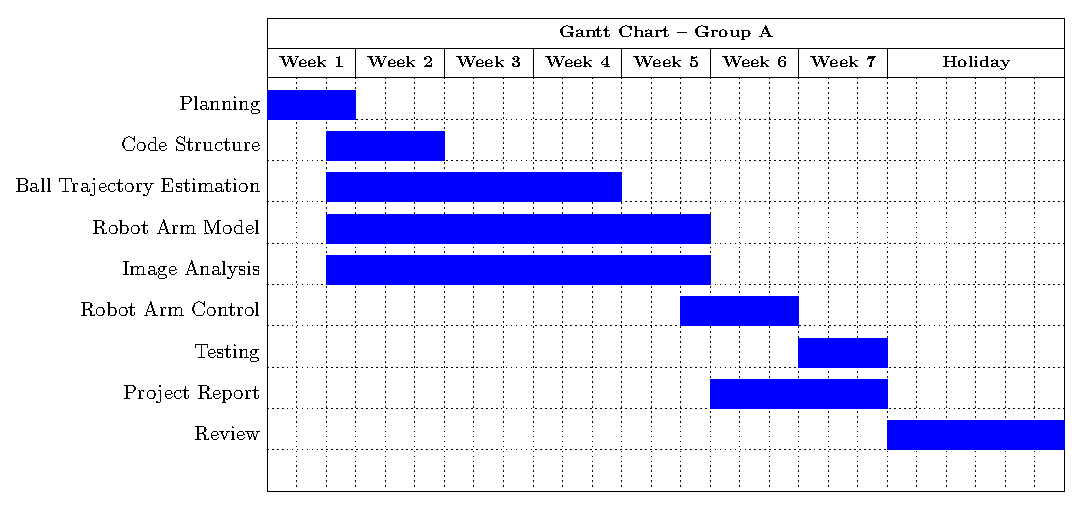
\includegraphics[width=0.95\textwidth]{figures/gantt}
        \caption{The Gantt chart describing the work flow of our project.}
        \label{fig:gantt}
    \end{figure}

\end{document}
